This section explains why we are focused exactly on the static analysis for Kotlin language.

Kotlin is a cross-platform, statically typed, general-purpose programming language with type inference. Kotlin is designed to interoperate fully with Java, and the JVM version of Kotlin's standard library depends on the Java Class Library, but type inference allows its syntax to be more concise. This language can be called "Java on steroids" as it takes best features from different languages and puts it on the top of JVM-world. Kotlin mainly targets the JVM, but also is compiled to JavaScript (e.g. for frontend web applications using React or Thymeleaf) or native code (via LLVM), e.g. for native iOS apps sharing business logic with Android apps. % wikipedia

Kotlin has quickly skyrocketed in popularity. It's used by Google, Square, Pinterest, Pivotal, Netflix, Atlassian and many other companies. It's the fastest-growing programming language, according to GitHub, growing over 2,5 times in the past year (2019). It was voted one of the five most loved languages, according to Stack Overflow. There are even meetups and conferences focused only on Kotlin\footnote{\url{https://www.businessinsider.com/kotlin-programming-language-explained-popularity-2019-5\#:\~:text=Kotlin\%20has\%20quickly\%20skyrocketed\%20in,times\%20in\%20the\%20past\%20year}}.
% https://www.businessinsider.com/kotlin-programming-language-explained-popularity-2019-5#:~:text=Kotlin%20has%20quickly%20skyrocketed%20in,times%20in%20the%20past%20year

Kotlin is used in a lot of ways. For example, it can be used for backend development using \texttt{ktor} framework (Kotlin framework developed by JetBrains), and  \texttt{Spring} framework that also has first-party support for kotlin (\texttt{Spring} is one of the most popular framework on Java for Web development). Kotlin/JS provides the ability to transpile your Kotlin code to JavaScript, as well as providing JS variant of Kotlin standard library and interopability with existing JS dependencies, both for Node.js and browser. There are numerous ways how Kotlin/JS can be used. For instance, Kotlin/JS is used to create frontend web applications, server-side and serverless applications, libraries for use with JavaScript and TypeScript.

Support for multiplatform programming is one of key benefits. It reduces time for writing and maintaining the same code for different platforms while retaining the flexibility and benefits of native programming. We think that it is the main reason why Kotlin is so popular in the community of mobile developers.

Kotlin supports well asynchronous or non-blocking programming. Whether we're creating server-side, desktop or mobile applications, it's important that we provide an experience that is not only fluid from the user's perspective, but scalable when needed. Kotlin has chosen a very flexible approach one by providing Coroutine support as a first-party library  \texttt{kotlinx.coroutines} with a kotlin compiler plugin. A coroutine is a concurrent design pattern that you can use on Android to simplify code that executes asynchronously. Coroutines (in a form of kotlinx.coroutines library and kotlin compiler plugin) were added to Kotlin in version 1.3 and are based on established concepts from other languages. Also, coroutines do not only open the doors to an easy asynchronous programming in Kotlin, but also provide a wealth of other possibilities such as concurrency, actors, etc.

On Android, coroutines help to manage long-running tasks that might otherwise block the main thread and cause your app to become unresponsive. Over 50\% of professional developers who use coroutines have reported that productivity had increased. So designers of Kotlin made a correct decision. Coroutines help you to write cleaner and more concise code for your applications.

The state of Kotlin in the Q3 of 2020 (according to the latest Kotlin Census and statistical data):
\begin{itemize}
    \item 4,7 million users
    \item 65\% of users use Kotlin in production
    \item Kotlin is primary language for 56\% of users, which means the main or only
    one they use at work
    \item 100+ people are on the Kotlin development team at JetBrains
    \item 350+ independent contributors develop the language and its ecosystem outside
    of JetBrains
\end{itemize}

% https://techcrunch.com/2019/05/07/kotlin-is-now-googles-preferred-language-for-android-app-development/
Kotlin is used by developers of open-source operating systems like HarmonyOS and Android. In 2019 Google announced that the Kotlin programming language is now its preferred language for Android app developers. In the same year Stack Overflow stated that Kotlin is fourth most loved language in community. Nowadays there are over 60\% of android developers who use Kotlin as their main language. \footnote{\url{https://techcrunch.com/2019/05/07/kotlin-is-now-googles-preferred-language-for-android-app-development/}}

Kotlin's popularity can be explained by the rising number of Android users (last year, 124.4m in the USA) and, thus, Android-based devices. 80\% of Kotlin programmers use the language to build Android apps, 31\% for back-end applications, 30\% for SDK/libraries.
Kotlin is also interoperable with Java, which allows developers to use all existing Android libraries in a Kotlin app. Now (2020) Kotlin is in the top-10 of PYPL rating:

\begin{figure}[H]
    \centering
    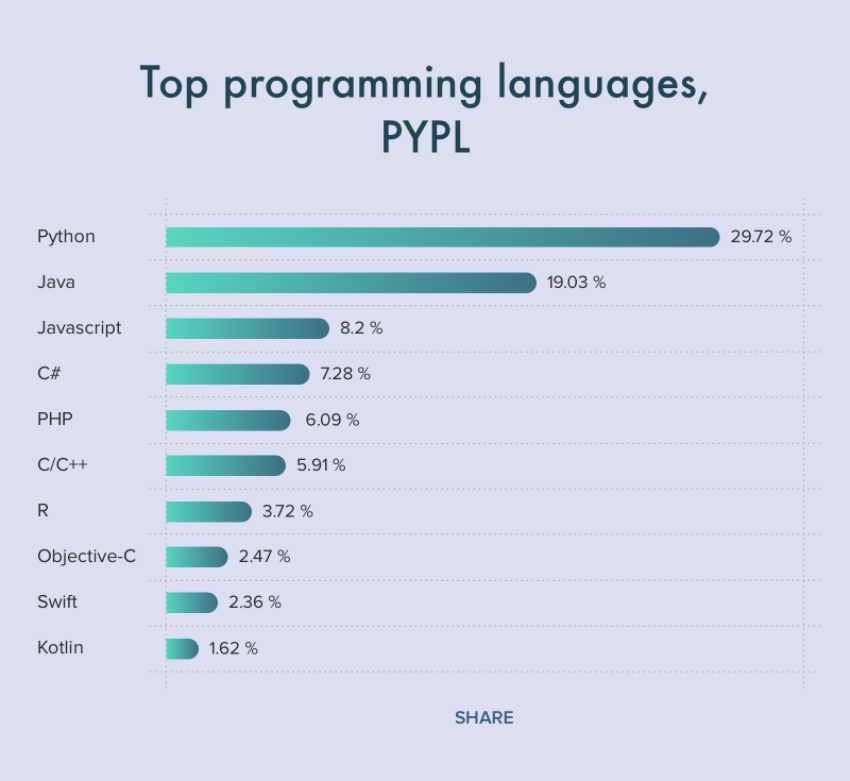
\includegraphics[scale = 0.3]{pictures/kotlinRating.png}
    \caption{Top programming languages, 2020}
    \label{fig:top_languages}
\end{figure}

Overall, Kotlin is a modern language that gains its popularity incredibly fast. It is mostly used by Android developers, but other "branches of programming" are gaining popularity as well, for example Spring framework (the most popular Java framework) supports Kotlin. It supports both OO (object-oriented) and FP (function-oriented) programming paradigms. Since the release 1.4 Kotlin claims to bring major updates every 6 month.